\documentclass[11pt,]{article}
\usepackage[left=1in,top=1in,right=1in,bottom=1in]{geometry}
\newcommand*{\authorfont}{\fontfamily{phv}\selectfont}
\usepackage[]{mathpazo}


  \usepackage[T1]{fontenc}
  \usepackage[utf8]{inputenc}



\usepackage{abstract}
\renewcommand{\abstractname}{}    % clear the title
\renewcommand{\absnamepos}{empty} % originally center

\renewenvironment{abstract}
 {{%
    \setlength{\leftmargin}{0mm}
    \setlength{\rightmargin}{\leftmargin}%
  }%
  \relax}
 {\endlist}

\makeatletter
\def\@maketitle{%
  \newpage
%  \null
%  \vskip 2em%
%  \begin{center}%
  \let \footnote \thanks
    {\fontsize{18}{20}\selectfont\raggedright  \setlength{\parindent}{0pt} \@title \par}%
}
%\fi
\makeatother




\setcounter{secnumdepth}{3}


\usepackage{graphicx,grffile}
\makeatletter
\def\maxwidth{\ifdim\Gin@nat@width>\linewidth\linewidth\else\Gin@nat@width\fi}
\def\maxheight{\ifdim\Gin@nat@height>\textheight\textheight\else\Gin@nat@height\fi}
\makeatother
% Scale images if necessary, so that they will not overflow the page
% margins by default, and it is still possible to overwrite the defaults
% using explicit options in \includegraphics[width, height, ...]{}
\setkeys{Gin}{width=\maxwidth,height=\maxheight,keepaspectratio}

\title{Descripción de Nidos de Hormigas UASD  }



\author{\Large Dahiana Guzmán Báez\vspace{0.05in} \newline\normalsize\emph{Estudiante, Universidad Autónoma de Santo Domingo (UASD)}  }


\date{}

\usepackage{titlesec}

\titleformat*{\section}{\normalsize\bfseries}
\titleformat*{\subsection}{\normalsize\itshape}
\titleformat*{\subsubsection}{\normalsize\itshape}
\titleformat*{\paragraph}{\normalsize\itshape}
\titleformat*{\subparagraph}{\normalsize\itshape}

\titlespacing{\section}
{0pt}{36pt}{0pt}
\titlespacing{\subsection}
{0pt}{36pt}{0pt}
\titlespacing{\subsubsection}
{0pt}{36pt}{0pt}





\newtheorem{hypothesis}{Hypothesis}
\usepackage{setspace}

\makeatletter
\@ifpackageloaded{hyperref}{}{%
\ifxetex
  \PassOptionsToPackage{hyphens}{url}\usepackage[setpagesize=false, % page size defined by xetex
              unicode=false, % unicode breaks when used with xetex
              xetex]{hyperref}
\else
  \PassOptionsToPackage{hyphens}{url}\usepackage[unicode=true]{hyperref}
\fi
}

\@ifpackageloaded{color}{
    \PassOptionsToPackage{usenames,dvipsnames}{color}
}{%
    \usepackage[usenames,dvipsnames]{color}
}
\makeatother
\hypersetup{breaklinks=true,
            bookmarks=true,
            pdfauthor={Dahiana Guzmán Báez (Estudiante, Universidad Autónoma de Santo Domingo (UASD))},
             pdfkeywords = {Ecología, nidos},  
            pdftitle={Descripción de Nidos de Hormigas UASD},
            colorlinks=true,
            citecolor=blue,
            urlcolor=blue,
            linkcolor=magenta,
            pdfborder={0 0 0}}
\urlstyle{same}  % don't use monospace font for urls

% set default figure placement to htbp
\makeatletter
\def\fps@figure{htbp}
\makeatother

\usepackage{pdflscape} \newcommand{\blandscape}{\begin{landscape}}
\newcommand{\elandscape}{\end{landscape}}


% add tightlist ----------
\providecommand{\tightlist}{%
\setlength{\itemsep}{0pt}\setlength{\parskip}{0pt}}

\begin{document}
	
% \pagenumbering{arabic}% resets `page` counter to 1 
%
% \maketitle

{% \usefont{T1}{pnc}{m}{n}
\setlength{\parindent}{0pt}
\thispagestyle{plain}
{\fontsize{18}{20}\selectfont\raggedright 
\maketitle  % title \par  

}

{
   \vskip 13.5pt\relax \normalsize\fontsize{11}{12} 
\textbf{\authorfont Dahiana Guzmán Báez} \hskip 15pt \emph{\small Estudiante, Universidad Autónoma de Santo Domingo (UASD)}   

}

}






\vskip 6.5pt


\noindent  \section{Introducción}\label{introducciuxf3n}

Las hormigas juegan un rol muy importante en el desarrollo de los
ambientes urbanos, estas pueden afectar de manera directa o indirecta a
muchos de lo seres vivos, como plantas y animales. Estas afecciones
pueden ser picaduras o mordeduras estas introduccen ácido fórmico en el
cuerpo de algunos animales causandole alergia. También dañan
edificaciones, alimentos, jardines y algunas pueden ser vectores de
agentes infecciosos (Klotz, Hansen, Pospischil, \& Rust, 2008; Robinson,
2005; Robinson \& others, 1996).

Las hormigas pertenecen al reino Animalia, filo Arthropoda, clase
Insecta, orden Hymenoptera y se distinguen de los demas animales por por
pertener a una única familia Formicidae. Se conocen alrededor de 12,000
a 20,000 especies de hormigas en el mundo, estas son clasificadas en
subfamilias (Chacón de Ulloa et al., 2008). En la hispaniola existen 43
géneros y 147 especies (\emph{Ants of hispaniola}, n.d.).

Las hormigas son seres vivos muy peculiares y apesar de esto se reunen
en grupos de especies a los cuales se le llaman gremios, cada gremio
comparten similitudes diferentes, como aspectos de su biología,
preferencia de hábitats y nichos; ejemplo de un gremio que ocupa de
forma exclusiva un nicho son las cultivadoras de hongos, todas las
hormigas de la tribu Attini (Chacón de Ulloa et al., 2008).

En esta investigación tomamos en cuenta la Ecología de nidos en la
Universidad Autonoma de Santo Dominingo. El nido es la parte fundamental
de la sociedad de hormigas. Cerca del 80-90\% de los miembros de una
colonia pertenecen en el nido (Petal, 1978). La arquitectura de los
nidos es muy variada, todo depende las especies que habiten en el nido.
Existen generos de hormigas que habitan ante todo en el suelo,
hojarasca, troncos o incluso en otros animales, por ejemplo Wasmannia
auropunctata y Paratrechina fulva (I. Armbrecht \& Ulloa-Chacón, 2003,
Zenner-Polania (1990)).

La ubicación de los nidos depende de los factores ambientales como
temperatura y humedad, también depende de la facilidad de reclutamiento
de alimentos para poder sobrevivir y reproducirse exitosamente Bernstein
\& Gobbel (1979).

Los nidos de hormigas y su modo de distribución en el espacio nos dan
información complementaría en el estudio de la comunidad en si. Por esa
razón para realizar esta investigación se tomaron en cuenta las
siguientes preguntas:

1- ¿Cuál es la distribución espacial entre los nidos edificado y
pavimentado que superan los 5 metros de distancia?

2- ¿Influye el transito de humanos en la diversidad de hormigas?

3- ¿Existe diferencia significativa en la densidad de nidos entre
distintos sustratos?

4- ¿Qué tanto recambio de especies existe entre nidos de sustratos
herbáceos o áreas contruidas?

\section{Metodología}\label{metodologuxeda}

\emph{Área de Estudio}

El trabajo se realizó en el campo de la Universidad Autonoma de Santo
Domingo (UASD) (18 27 40 N, 69 55 02 W). Tiene un área aproximada de
375, 000 m. Limita al norte con la Av. José Contreras, al sur con la Av.
Correa y Cidrón, al este con la Av. Santo Tomás de Aquino, y al oeste
con la calle General Modesto Diaz. Posee una temperatura promedio anual
de 25.7 C. Eligimos está área porque tiene un fácil acceso y por poseer
diferentes tipos de sustratos o coberturas como herbaceos, dosel,
construido, edificados, no edificado ni cubierto, entre otros. Además en
esta área existe una gran diversidad de hormigas.

\begin{figure}
\centering
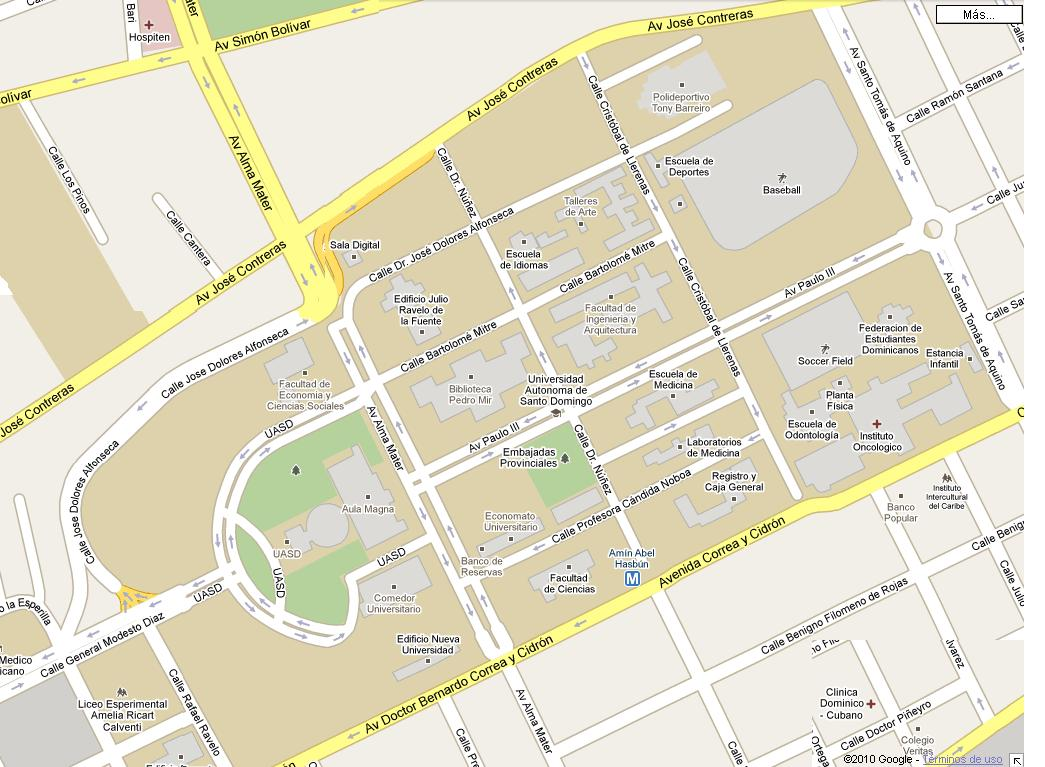
\includegraphics{uasd.jpg}
\caption{Mapa de la Universidad Autonoma de Santo Domingo, imagen
extraída de Google imagenes.}
\end{figure}

\emph{Materiales y métodos}

\begin{figure}
\centering
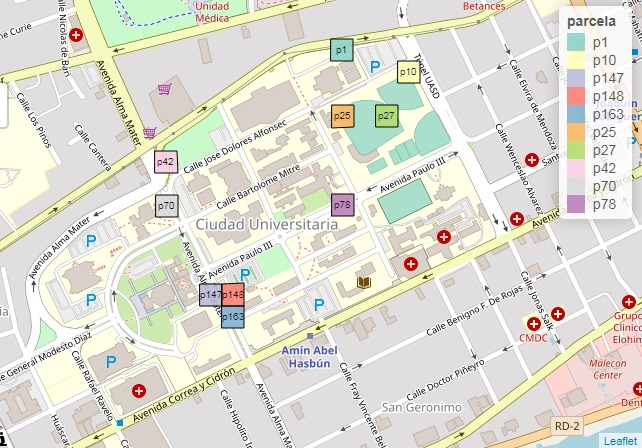
\includegraphics{parcelas estudiadas.jpg}
\caption{Mapa de las parcelas estudiadas.}
\end{figure}

{[}Se seleccionarion un total de 10 parcelas establecidas para el campo
de la UASD con diferentes tipos de coberturas, construido, mobiliario,
suelo, herbáceos, no edificado ni cubierto. Los muestreos fueron
realizados desde el día 12 al 26 de octubre del año 2019.

Entre los materiales que utilizamos estan: frascos plásticos, alcohol
etílico al 80\%, pinceles de cerdas claras, papel vegetal para las
etiquetas, chinográfo para escribir, dispositivo Android para llenar los
formulario de ODK Collect. ODK es un conjuntos de herramientas de código
libre que crea formularios para poder recoger los datos en un
dispositivo móvil y enviarlos a un servido.

Como se menciono anteriormente esta investigación se basó en la ecología
de nidos. Para realizar la coleccón de datos se hizo un censo detallado
de nido en cada parcela, tomando datos dentro de la cobertura que le
corresponde a la parcela elegida. Luego se toman las coordenas de cada
nido, información ambiental y relación de flora asociada al nido.

En cada nido se colecto de 5 a 8 individuos, para hacerlo utilizamos un
pincel humedicido con alcohol etílico al 80\%, luego cada individuo de
un mismo nido se deposito en un mismo frasco, es decir. Se utilizo un
frasco por nido el cual estaba debidamente etiquetado en papel vegetal
el nombre del colector, fecha y hora, el número de la parcela y la
muestra (p\#m\#). El trabajo de campo fue realizado por dos personas,
una relleno el formulario de ODK y la otra colecto las hormigas. Por
último pero no menos importante, los formularios fueron enviados a un
servidor para ser evaluados.

Culminado con la recolección de datos del campo, el siguiente paso fue
realizar la identificación de cada individuo encontrado en cada nido.
Para esto se utilizo una lupa de modelo AmScope 3.5X-180X Inspection
Zoom Stereo Microscope +144-LED Light, pinzas, porta objetos, alcohol al
80\%, guía de identificación hasta género de hormigas utilizando la guía
de AntWiki y llenar los formularios para identificación de ODK.{]}

\section{Resultados}\label{resultados}

\begin{figure}
\centering
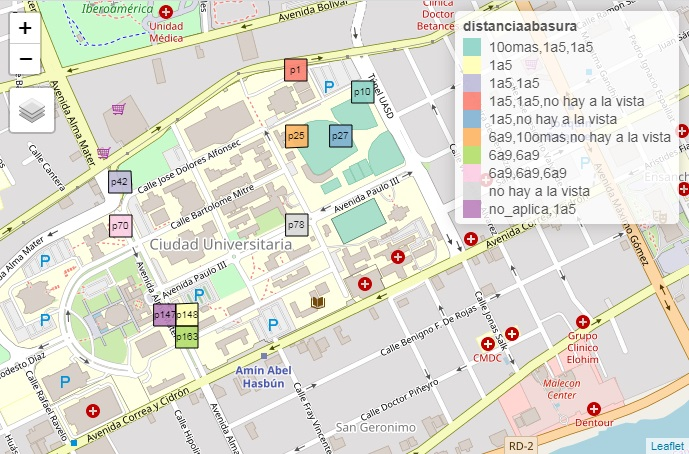
\includegraphics{distancia a basura.jpg}
\caption{Distancia a basura. Este mapa nos muestra la distancia a basura
que estan los nidos de cada parcela. Los nidos que menos distantes esten
de basura tienen mas diversidad, esto se debe a que pueden conseguir mas
facil sus alimentos, entre otras cosas; por ejemplo en la parcela p42 la
distancia a basura de los dos nidos encontrados fue de 1a5, por ende
esta parcela tiene una diversidad moderada ya que se encontraron dos
géneros diferente. Sin embargo, la parcela p78 no tuvo basura a la
vista, por ende tiene una poca diversida ya que solo se encontro un solo
género.}
\end{figure}

\begin{figure}
\centering
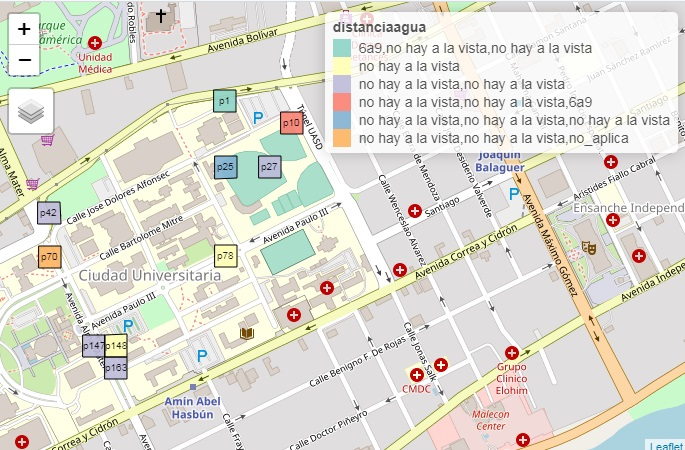
\includegraphics{distanciaagua.jpg}
\caption{Distancia a agua. Este mapa nos muestra la distancia a agua. El
agua es indispensable para la mayoría de los seres vivos y las hormigas
no son la excepción, pero sabemos que sus refugios son lejos del agua o
si llueven encuentran un lugar seguro donde no esten expuestas. Por esta
razón, en este estudio solo se encontraron dos parcela cerca de agua fue
la p1 Y p10; los nidos encontrados en estas parcelas algunos no tenía
agua a la vista y otros a una distancia de 6a9. Sin embargo, estas
parcela tenían una diversidad alta, por ejemplo en la parcela p1 se
encontraron dos géneros distintos y en la p10 3 géneros distintos.}
\end{figure}

\begin{figure}
\centering
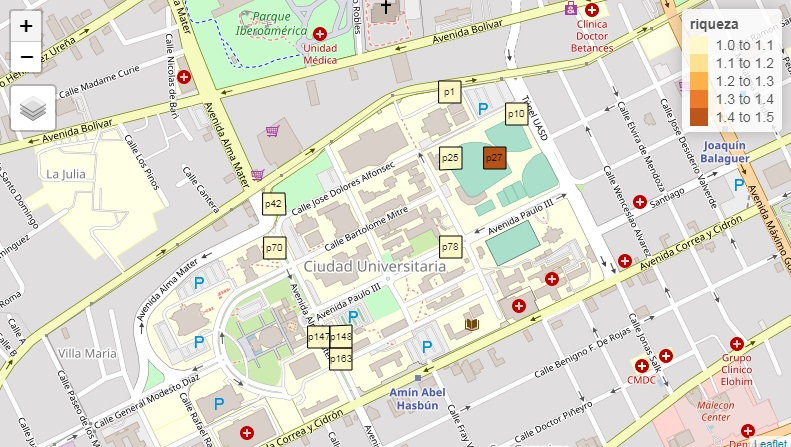
\includegraphics{riqueza.jpg}
\caption{Mapa de riquezaEn este mapa podemos observar la biodiversidad
en cada parcela. Este mapa nos muestra que la riqueza de géneros no es
homogenea, los patrones de diversidad pueden depender de varios
factores, como el tamaño del hábitat, de la productividad, la frecuencia
de las perturbaciones. En este estudio las parcelas mas diversas o mejor
dicho con mayor riqueza son las p10 y p1, pero también se encontraron
parcelas con muy baja diversidad como son las p27 y p78.}
\end{figure}

\begin{figure}
\centering
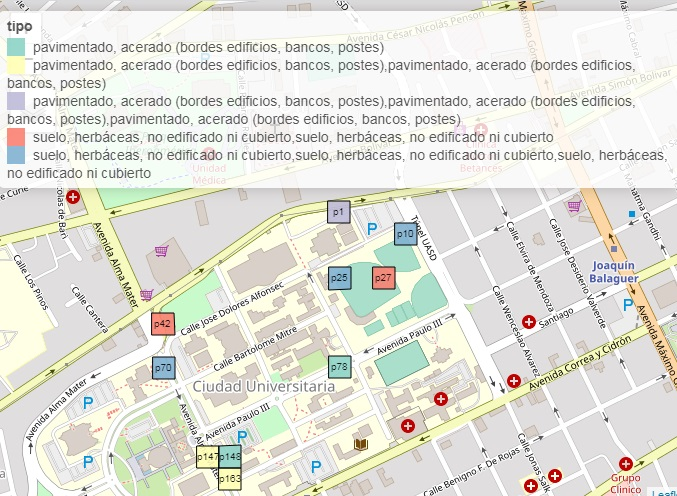
\includegraphics{sustrato.jpg}
\caption{Mapa de sustrato. Este mapa nos muestra los diferentes
sustratos que se estudiaron. El sustrato es una variable fundamental en
la diversidad de individuos, ya que cada especie tiene su hábitat
específico para desarrollarse con exito, sin embargo existen sustrato
con mayor diversidad que otros, ya sea por tener mejor tasa de alimentos
y ser menos propensos a perturbaciones. Es común que los suelos
herbacios, no edificados ni cubiertos esten mas poblado que otros
sustrato. Por ejemplo las parcelas p10 y p25 tiene el sustrato
mencionado anteriormente y en estas parcelas existe una mayor diversidad
de género que en los demás sustratos.}
\end{figure}

\begin{figure}
\centering
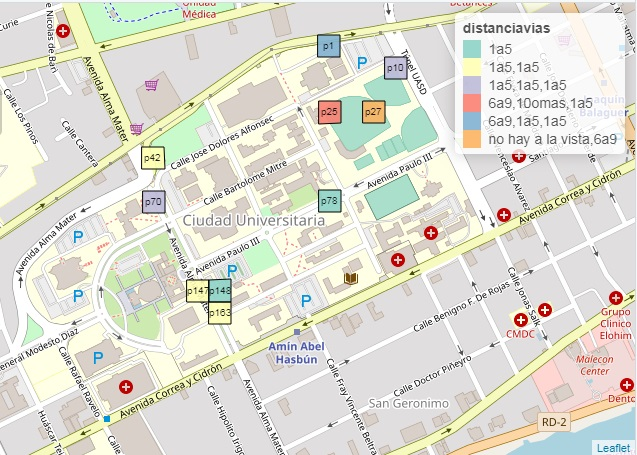
\includegraphics{distanciavias.jpg}
\caption{En este mapa podemos observar la distancia en metros a que
estan las vías de los nidos dentro de una parcela. Las parcelas que
obtuvieron mayor diversidad de nidos estan a una distancia considerada
de las vía o aseras como por ejemplo las parcelas p10, p25 y p27 ya que
están menos propensas a pertubaciones (ir a la figura 9).}
\end{figure}

\begin{figure}
\centering
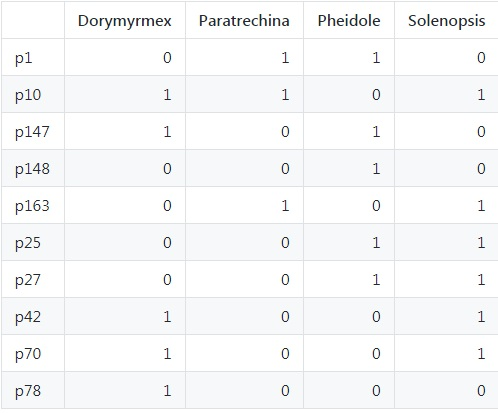
\includegraphics{generos por parcela.jpg}
\caption{Tabla de los géneros encontrados. Esta tabla nos muestra los
generos encontrados en cada parcela, como podemos observar existen dos
parcelas exclusiva en la cuales solo se encontro un género en todos lo
nidos estudiado que son el género Dorymyrmex y Pheidole, a diferencia de
las demás parcelas que comparten mas de dos géneros diferentes.}
\end{figure}

\begin{figure}
\centering
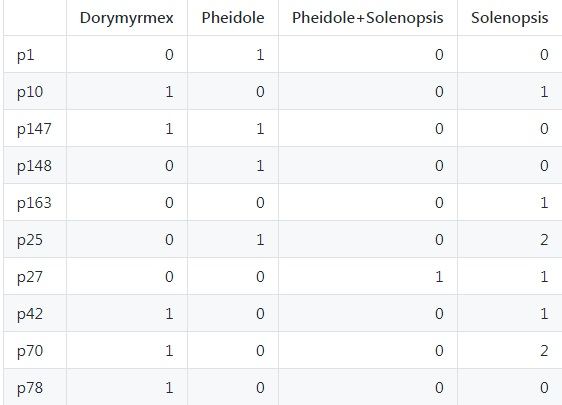
\includegraphics{similtud.jpg}
\caption{Tabla de los géneros encontrados. En esta tabla podemos
observar una ``rareza'', ya que se encontro en la parcela p27 dos
géneros diferentes en un mismo nido, esto solo ocurrió en esta parcela,
en las demás cada nido encontrado estaba compuesto por individuos del
mismo género.}
\end{figure}

\begin{figure}
\centering
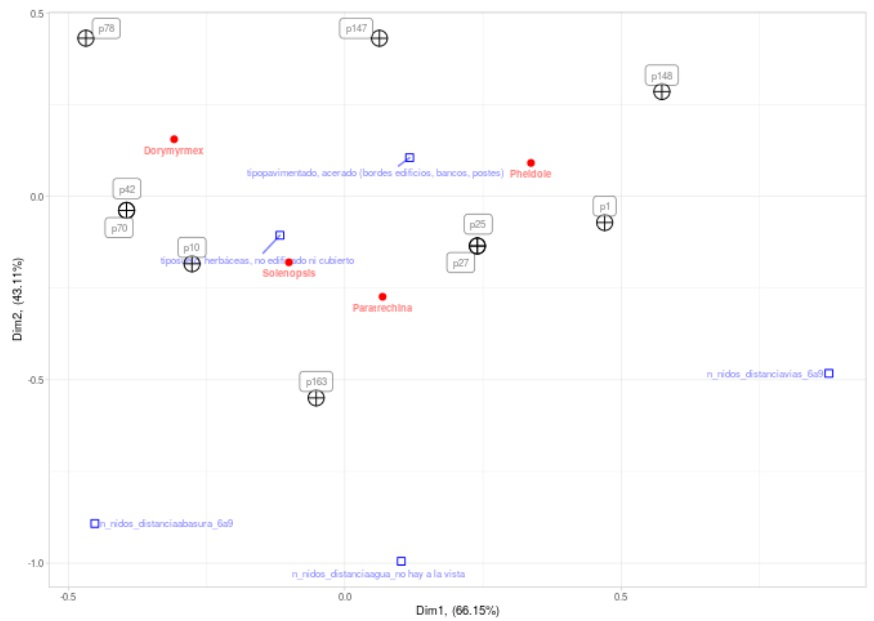
\includegraphics{biplot.jpg}
\caption{Gráfico de Biplot. El gráfico biblot explica la relación que
existe entre los objetos dentro de de la muestra; en este caso los
objetos son: géneros (representado con un punto rojo), sitios
(representado con con un circulo) y variables (representado con un
cuadrado). Además este gráfico consta de dos dimensiones, como podemos
ver en el gráfico existe una extrecha relación entre el género
Solenopsis y la varible tipo herbaseos, no edificado ni cubierto.}
\end{figure}

\begin{figure}
\centering
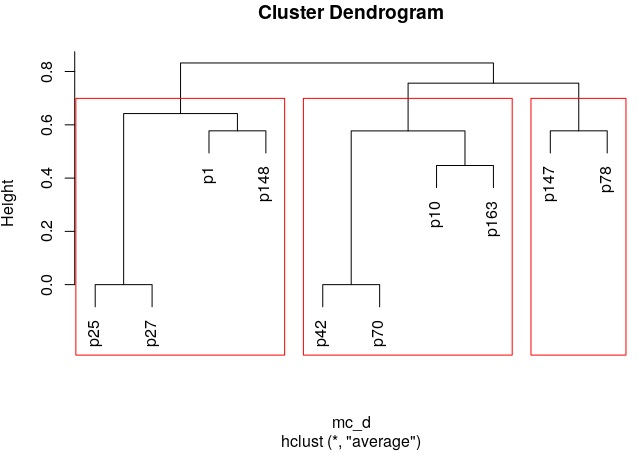
\includegraphics{dendograma.jpg}
\caption{Gráfico dendograma. Este gráfico muestra un anális Cluster, el
cual funciona para agrupar elementos (o variables) tratando de lograr la
máxima homogeneidad en cada grupo y la mayor diferencia entre los
grupos. Por ejemplo en este gráfico podemos ver que las parcelas p25 y
27 estan a la misma altura por lo tanto forma un clado que a su vez esta
en el mismo grupo del clado formado por las parcelas p1y p48, en general
este grupo alcanza su máxima homegeneidad y es diferentes a los otros.}
\end{figure}

\begin{figure}
\centering
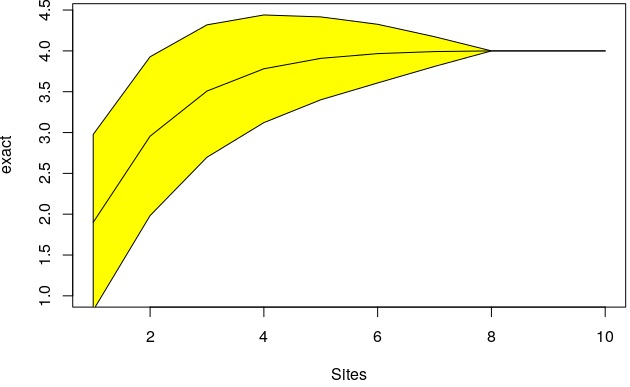
\includegraphics{grafico amarillo.jpg}
\caption{Las curvas de acumulación de especies es una representación
gráfica del número de especies presentes en el sitio de estudio, en este
gráfico podemos ver que existe una relación directa entre las dos
variables, ya que si una aumenta la otra aumenta en la misma proporción
hasta llegar a un punto donde va rápdio y luego se estabiliza.}
\end{figure}

\begin{figure}
\centering
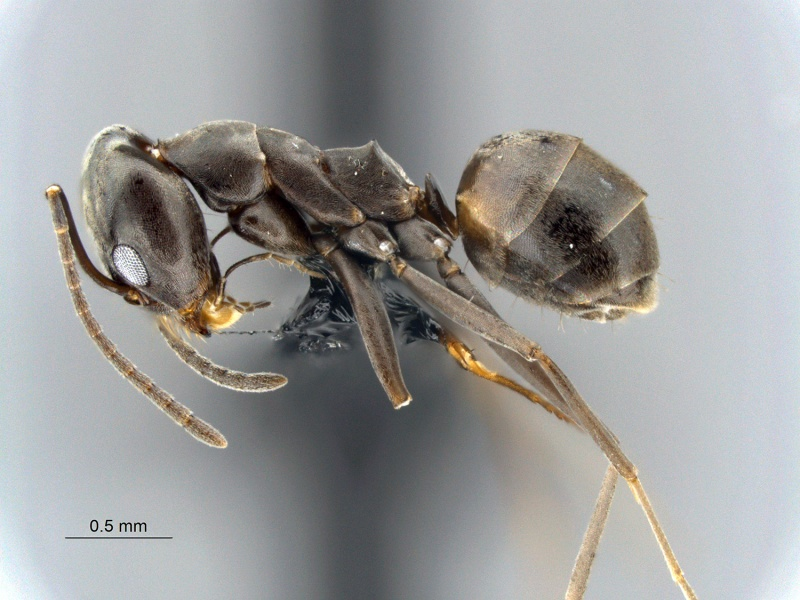
\includegraphics{dorymyrmex.jpg}
\caption{Imagen de Dorymyrmex sp. Una de las especies identificada en
esta investigación}
\end{figure}

\begin{figure}
\centering
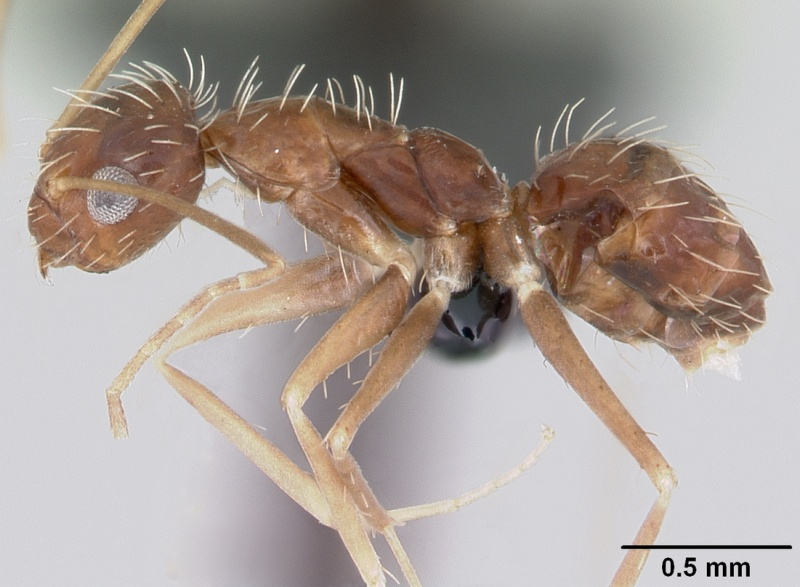
\includegraphics{paratrechina.jpg}
\caption{Imagen de Paratrechina sp. Una de las especies identificada en
esta investigación.}
\end{figure}

\begin{figure}
\centering
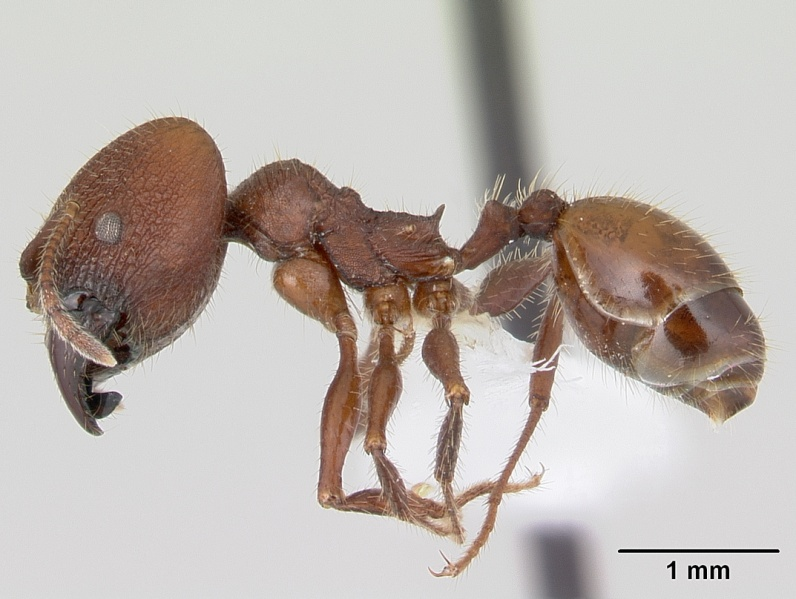
\includegraphics{pheidole.jpg}
\caption{Imagen de Pheidole sp. Una de las especies identificada en esta
investigación.}
\end{figure}

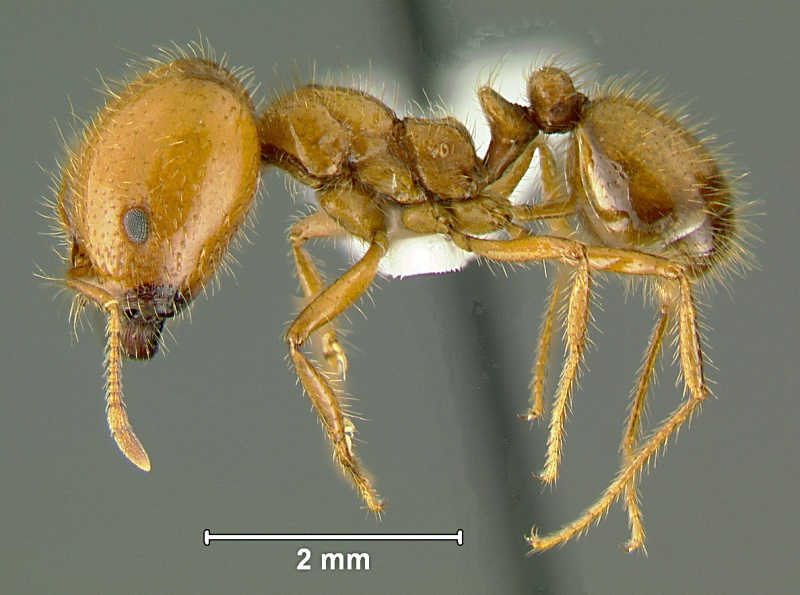
\includegraphics{solenopsis.jpg} {]}

\section{Discusión}\label{discusiuxf3n}

Es importante destacar que existe una amplia diferencia entre las
parcelas situadas en edicaciones y las situadas en pavimentado; En los
bordes de las edificaciones se encontraron muy pocos nidos, sin embargo,
en las grietas del suelo pavimentado era muy común encontrar varios
nidos, y más común si cerca existía un deposito de basura, además los
nidos encontrados en pavimento superar una distancia de 5 metros de los
nidos encontrados en edificaciones que casi nunca existía deposito de
basura cerca. Dicho esto, se puede concluir que las parcelas que cuentan
con almacenamiento de basura cerca de este es posible encontrar nidos y
en su gran mayoría la parcela puede tener una gran diversidad de
individuos.

El transito de humanos o la distancia a vías son uno de los factores que
mas influye en la diversidad de las hormigas. Por ejemplo en este
estudio las parcelas que mas alejadas estuvieron de las vías o del flujo
de personas se encontraron más nidos, ya que están menos propensas a
perturbaciones y pueden andar en su hábitat libremente (ir a la figura
8).

El sustrato es otro de los factores indispensable al momento de estudiar
hormigas, el tipo de sustrato puede decirnos rapidamente la
heterogeniedad que existe en una área. Como ejemplo de esto tenemos el
sustrato tipo herbáceos, en este estudio fue en el que más nidos se
encontro y el que mayor diversidad de individuos represento. En pocas
palabras los suelos herbácios presentan una densidad mayor que el
sustrato pavimentado o edificado. Es importante destacar que no existe
un gran recambio de especie según el sustrato, esto fue demostrado ya
que se encontraron géneros iguales en sustratos diferentes.

En este trabajo uno de los géneros más encontrado en los nidos fueron
las especies del género Pheidole, presente en 5 parcelas, siguiendole a
esta las especies del género Solenopsis presentes en 6 parcelas. En un
estudio realizado en México la especie más encontrada fue del género
Pheidole con un total de 51 individuos, presente en diferentes sustratos
(P. R. Fernández, 2001).

{]}

\section{Agradecimientos}\label{agradecimientos}

Al profesor José Ramón Martinez Batlle, por impartir esta asignatura y
brindarnos su apoyo incondicional para mí aprendizaje y el de mis
compañeros.

A mi compañero Enrique García, por ayudarme en la colecta de hormihgas.

\section*{Referencias}\label{referencias}
\addcontentsline{toc}{section}{Referencias}

\hypertarget{refs}{}
\hypertarget{ref-AntWiki}{}
\emph{Ants of hispaniola}. (n.d.).
\url{http://www.antwiki.org/wiki/Ants_of_Hispaniola}.

\hypertarget{ref-armbrecht2003little}{}
Armbrecht, I., \& Ulloa-Chacón, P. (2003). The little fire ant wasmannia
auropunctata (roger)(Hymenoptera: Formicidae) as a diversity indicator
of ants in tropical dry forest fragments of colombia.
\emph{Environmental Entomology}, \emph{32}(3), 542--547.

\hypertarget{ref-bernstein1979partitioning}{}
Bernstein, R. A., \& Gobbel, M. (1979). Partitioning of space in
communities of ants. \emph{The Journal of Animal Ecology}, 931--942.

\hypertarget{ref-chacon2008aspectos}{}
Chacón de Ulloa, P., Armbrecht, I., Lozano-Zambrano, F., Jiménez, E.,
Fernández, F., \& Arias, T. (2008). Aspectos de la ecología de hormigas
cazadoras en bosques secos colombianos. \emph{Sistemática, Biogeografía
Y Conservación de Las Hormigas Cazadoras de Colombia}.

\hypertarget{ref-fernandez2001hormigas}{}
Fernández, P. R. (2001). Las hormigas del suelo en méxico: Diversidad,
distribución e importancia (hymenoptera: Formicidae). \emph{Acta
Zoológica Mexicana (Nueva Serie)}, (Es1), 189--238.

\hypertarget{ref-klotz2008urban}{}
Klotz, J. H., Hansen, L. D., Pospischil, R., \& Rust, M. (2008).
\emph{Urban ants of north america and europe: Identification, biology,
and management}. Cornell University Press.

\hypertarget{ref-petal1978role}{}
Petal, J. (1978). Role of ants in ecosystems. \emph{International
Biological Programme}.

\hypertarget{ref-robinson2005urban}{}
Robinson, W. H. (2005). \emph{Urban insects and arachnids: A handbook of
urban entomology}. Cambridge University Press.

\hypertarget{ref-robinson1996urban}{}
Robinson, W. H., \& others. (1996). \emph{Urban entomology: Insect and
mite pests in the human environment.} Chapman \& Hall.

\hypertarget{ref-zenner1990biological}{}
Zenner-Polania, I. (1990). Biological aspects of the ``hormiga loca'',
paratrechina (nylanderia) fulva (mayr). \emph{Colombia. in: Vander Meer
RK, Jaffe K, Cedeno A (Ed) Applied Myrmecology: A World Perspective.
Westview Press, Boulder}, 290--297.




\newpage
\singlespacing 
\end{document}
